%!TEX root = Main.tex
\documentclass[Main]{subfiles}

\begin{document}

\section{Design And Implementation} % (fold)
\label{sec:design_and_implementation}

	\subsection{Data Input} % (fold)
	\label{sub:data_input}

		The MATLAB script \texttt{InputData.m} uses build in functions to extract data from the downloaded G1SST database.
		It takes as input an upper and lower bound and an eastern and western bound in between which it is supposed to a square set of data.

		The data is converted from Kelvin to Celsius, to make it more semantically understandable.
		The data is then saved to a \texttt{.mat}-file for use in other scripts.

		Finally the data is shown on a colored contour-plot (see Figure \ref{fig:ExampleSSTData}), for illustration and inspection purposes.

	
		% subsection data_input (end)

	\subsection{Sparsity Estimation} % (fold)
	\label{sub:sparsity_estimation}

		The MATLAB script \texttt{EvalSparsity.m} takes as input to \emph{.mat}-file described in Section \ref{sub:data_input}.

		It vectorizes the data map by stacking either the rows or the columns.
		The snake pattern, described in Section \ref{par:vectorization_of_data_map} is also implemented, and is enabled by a boolean \texttt{snake}.

		Then it evaluates the sparsity by taking either the DFT or the DCT of the signal.
		The sparsity is the number, $k$, of coefficients greater than 10 or 0.1, respectively.
		It then tries to do a reconstruction using $M = 6*k$ randomly selected samples, and calculates the normalized error:
		%
		\begin{equation}
			e_{normalized} = \frac
				{\|\mathbf{\hat{u}}(n) - \mathbf{u}(n)\|_{l2}}
				{\|\mathbf{u}(n)\|_{l2}}
		\end{equation}

		In Figure \ref{fig:ExEvalSparseSnakeOff} below the result of running the script on data from a patch of the North Sea.
		The data is visibly sparse, in the sense that most of the energy in the DCT is confined to at small number of coefficients.
		The power does however not taper off as rapidly as one would like.
		Especially, there are some powerful harmonics present.

		When \texttt{snake} is set to \texttt{true}, enabling the use of the snake pattern, the amount of harmonic overtones present is greatly reduced, as seen in Figure \ref{fig:ExEvalSparseSnakeOn}.
		This results in much greater performance, as the level of error is maintained while the number of samples used is \emph{reduced to one third}. 

		Another way of determining the sufficient number of samples, $N_S$ required for reconstruction is by doing is experimentally.
		This process entails attempting reconstruction with an increasing number of samples available, and seeing when the error has decreased enough.

		The MATLAB script \texttt{FindOptimumNs.m} does this.
		It goes trough the process of reconstructing the data from randomly selected data points, for a series of logarithmically spaced values of $M$, doing it 10 times for each value and averaging the result.
		This produces a plot like the on shown in \ref{fig:Estimation_Ns}.
		This figure can then be used to give a good estimate of $N_s$.

		\begin{figure}[H]
			\centering 
			\includegraphics[width=\textwidth]{ExEvalSparseSnakeOff.eps}
			\caption{
				Results of running \texttt{EvalSparsity.m} on a patch of data from the North Sea.}
			\label{fig:ExEvalSparseSnakeOff}
		\end{figure}

		\begin{figure}[H]
			\centering 
			\includegraphics[width=\textwidth]{ExEvalSparseSnakeOn.eps}
			\caption{
				Results of running \texttt{EvalSparsity.m} on a patch of data from the North Sea with snake pattern enabled.}
			\label{fig:ExEvalSparseSnakeOn}
		\end{figure}

		\begin{figure}[H]
			\centering 
			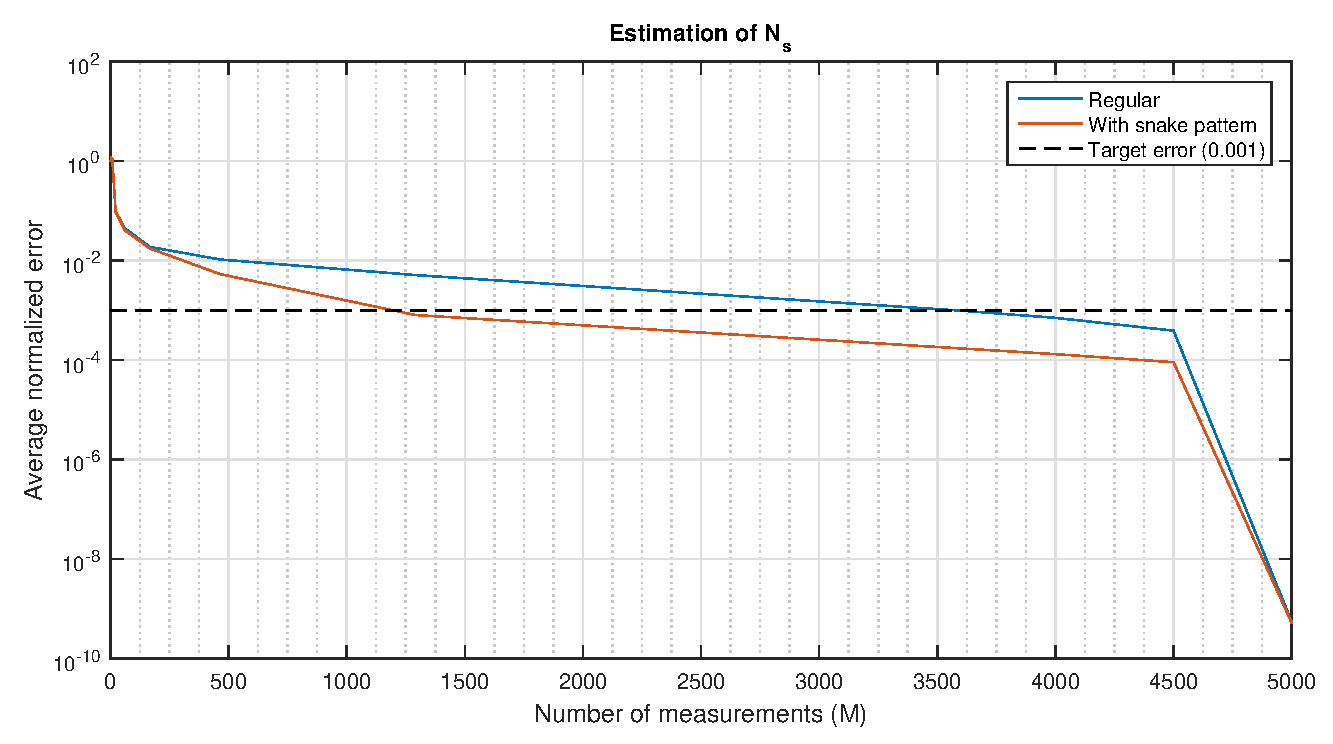
\includegraphics[width=\textwidth]{Estimation_Ns.eps}
			\caption{
				Results of running \texttt{FindOptimumNs.m} on a patch of data from the North Sea. The values of $N_s \approx 3500$ for the regular version and $N_S \approx 1100$ with the snake pattern match the calculations above.}
			\label{fig:Estimation_Ns}
		\end{figure}



	
		% subsection sparsity_estimation (end)

	\subsection{Estimaton of $q_s$ and $p_s$} % (fold)
	\label{sub:estimaton_of_q_s_and_p_s}

		With an estimate of $N_s$, you can now calculate the required sensing probability, $p_s$.
		This is done by the MATLAB script \texttt{SensingProbability.m}.
		It takes the network specifications (Probability of sufficient sensing $P_s$, Frame time $T$, Packet transmission time $T_p$ and Total number of sensors $N$) and $N_s$ as input.

		It first uses the Complementary Cumulative Distribution Function $Q_K(k)$ (see (\ref{eq:CCDF})) to numerically search for a $q_s$ that satisfies 
		%
		\begin{equation}
			Q_K(N_s) \geq P_s
		\end{equation}
		%
		as shown in Figure \ref{fig:q_s_Example}.

		\begin{figure}[H]
			\centering 
			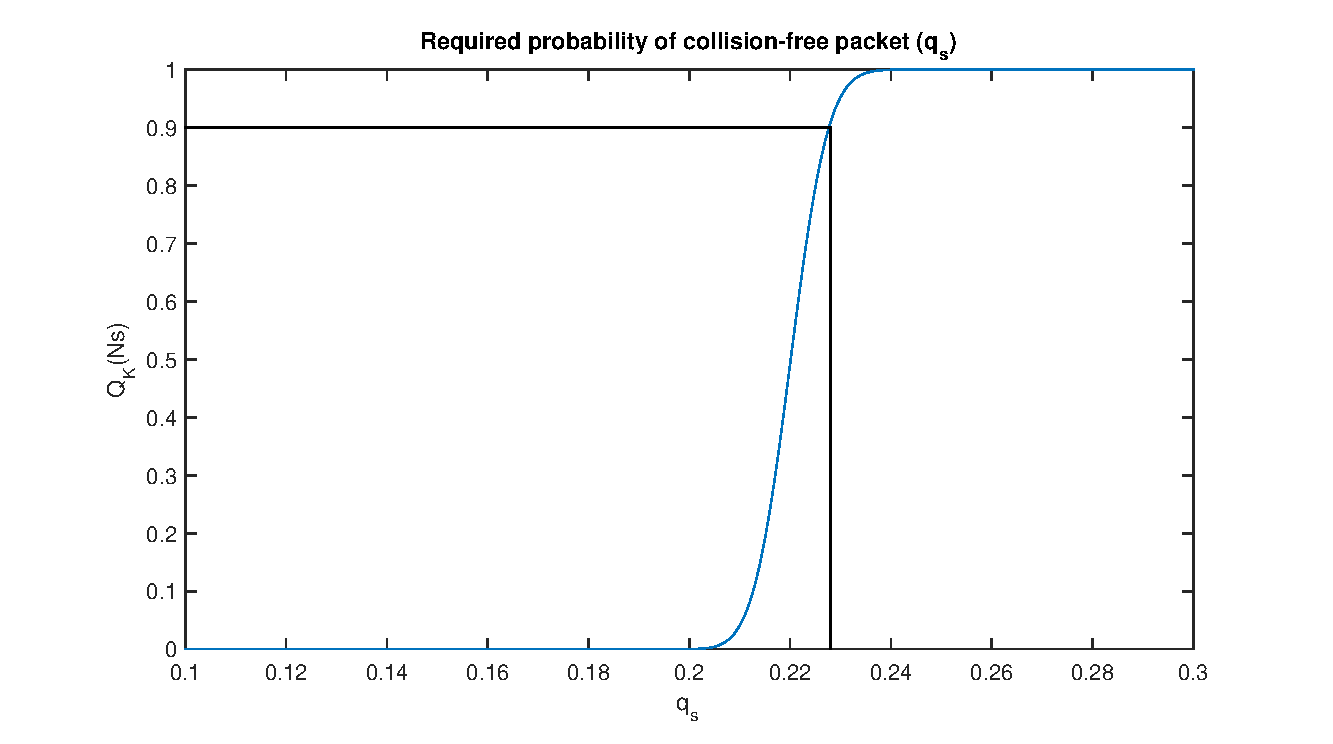
\includegraphics[width=0.8\textwidth]{q_s_Example.eps}
			\caption{
				Search for $q_s$ given: 
				$P_s = 0.90$, 
				$N = 5000$ and
				$N_s = 1100$ | 
				$q_s = 0.228$
			}
			\label{fig:q_s_Example}
		\end{figure}

		Then another numeric search is performed to find the minimum necessary $p_s$ that satisfies
		%
		\begin{equation}
			q_s =
				e^{
					-2\frac
						{Np_sT_p}
						{T-T_p}
					}
			\label{eq:qs_from_ps}
		\end{equation}
		%
		as shown in Figure \ref{fig:p_s_Example}.

		\begin{figure}[H]
			\centering 
			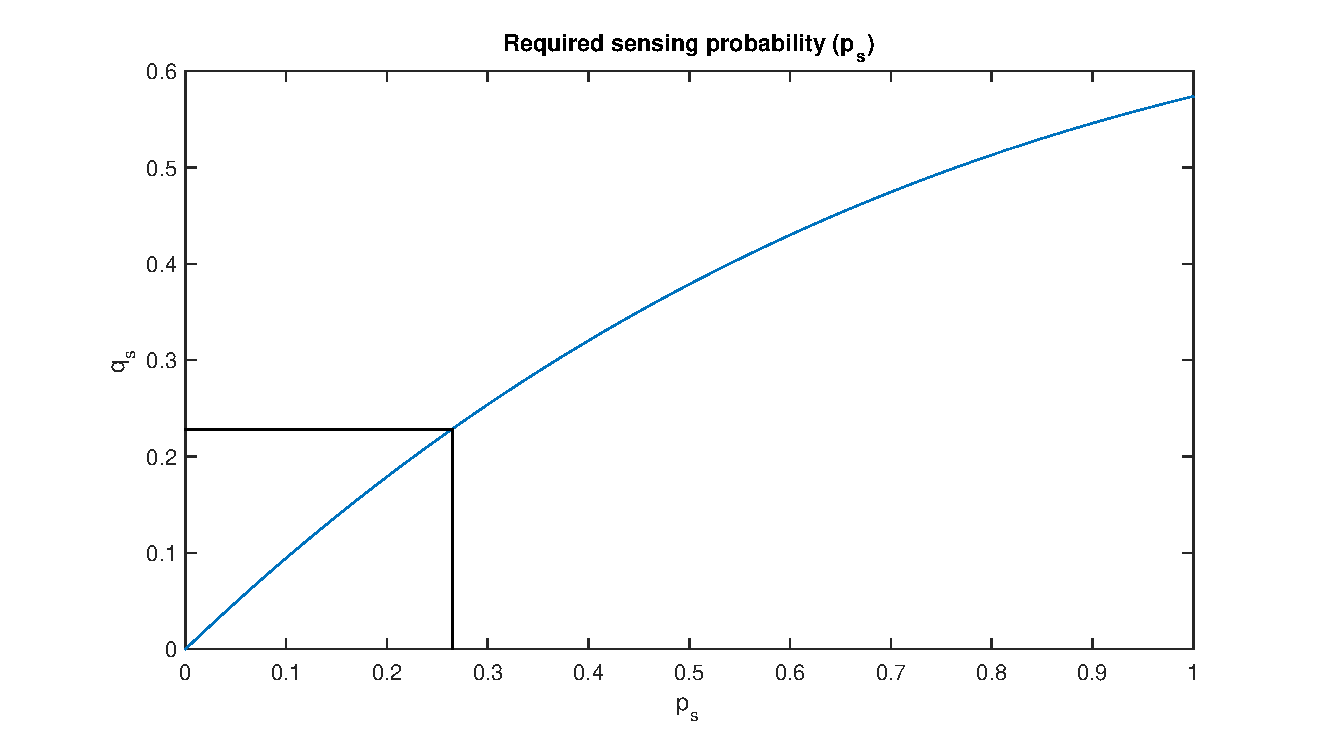
\includegraphics[width=0.8\textwidth]{p_s_Example.eps}
			\caption{
				Search for $p_s$ given:
				$q_s = 0.228$, 
				$T_p = 200\ ms$, 
				$T = 1\ hour = 3600\ s$  and
				$N = 5000$ |
				$p_s = 0.265$ 
			}
			\label{fig:p_s_Example}
		\end{figure}

		If a solution for (\ref{eq:qs_from_ps}) does not exits, it means that the probability of sufficient sensing is infeasible with the given bandwidth and frame time.
		In this case the script returns an error.

		% subsection estimaton_of_q_s_and_p_s_ (end)


	\subsection{Simulation of Random Access Transmission} % (fold)
	\label{sub:simulation_of_random_access_transmission}

		The MATALB function \texttt{TransmissionSimulation.m} simulates RACS random access protocol.
		It takes as input, The number of sensors $N$, the probability of sensing $p$, the packet transmission time $T_p$ and the frame period $T$.

		It does this by first selecting a random set of $M$ sensors for sensing.
		Each sensor selected for sensing is assigned a random time to start transmission $\theta_i$ distributed uniformly in the range $[0 ; T - T_p]$.

		All the indexes of the sensors selected for sensing are initially put in the set of received sensors.
		Then one-by-one for each selected sensor $i$ it is tested if 
		$\theta_i - T_p < \theta_j < \theta_i + T_p$
		for any
		$j \neq i$.
		If so, the index of sensor $i$ is removed from the set of received sensors.

		When all sensors have been tested for collision, the function returns a list of indexes of successfully received sensors $receiveIndex$, the number of sensors selected for sensing $M$ and the number of successfully received sensors $k$.

		In Figure \ref{fig:Mean_k_vs_p} below \texttt{TransmissionSimulation.m} is compared with the binomial model (\ref{eq:BinomialModel}) presented in Section \ref{sub:random_access}.

		\begin{figure}[H]
			\centering 
			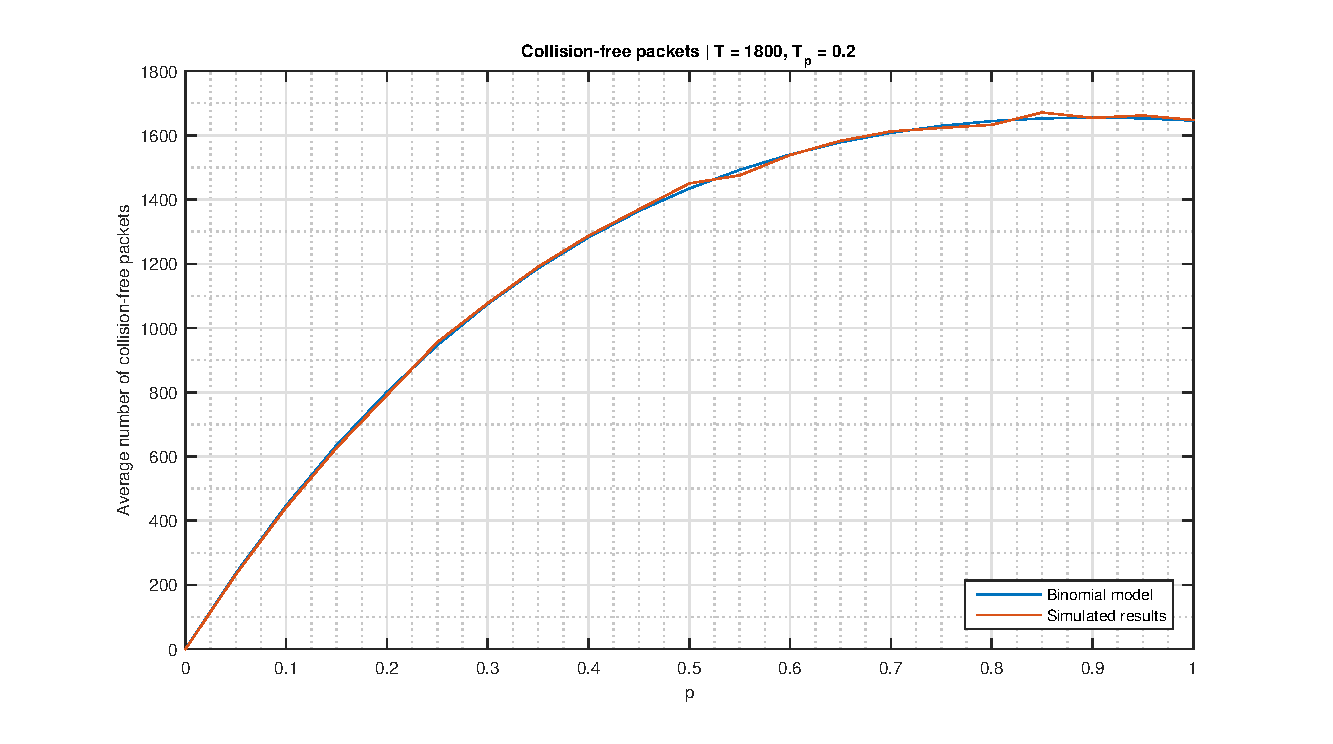
\includegraphics[width=\textwidth]{Mean_k_vs_p.eps}
			\caption{Comparison of \texttt{TransmissionSimulation.m} and binomial model. Averaged over 5 simulation runs.
			Number of sensors $N = 5000$.
			Frame time $T = 1800\ s = \sfrac{1}{2}\ hour$.
			Packet transmission time $T_p = 200\ ms$}
			\label{fig:Mean_k_vs_p}
		\end{figure}

		\fxnote{reconstruction error vs p figure}
	
		% subsection simulation_of_random_access_transmission (end)

	\subsection{Data Reconstruction (Sensor Fusion)} % (fold)
	\label{sub:data_reconstruction}

		Reconstructing data from a subset of all the data is a matter of solving the convex optimization problem (\ref{eq:minimizationProblem}) presented in Section \ref{sub:compressive_sensing_in_spatial_domain}.
		In this project this is done using the the MATLAB function \texttt{SolveBP.m} from the toolbox called Sparelab \cite{SparseLab:Online}.
		
		This function takes as input the augmented basis $\Phi'$, which is the selection matrix $R$ multiplied with the selected basis $\Psi$, the received vector $y$ and the total number of sensors $N$.
		It then uses the \emph{Basis Pursuit} method to solve the problem and returns a reconstructed vector.
		It is then only a matter of reshaping the vector back into a matrix, and you have the reconstructed data map.

	
		% subsection data_reconstruction (end)

	\subsection{Full Simulation} % (fold)
		\label{sub:full_simulation}

		The MATALB script \texttt{RACS\_Simulation.m} simulates a full RACS frame.
		It takes the network specifications (Probability of sufficient sensing $P_s$, Frame time $T$ and Packet transmission time $T_p$) and the data as input.
		Then it goes trough the entire process of estimating sparsity, determining probability of sensing $p_s$, simulating transmission, reconstructing the data map and calculating the normalized error.

		Finally the results are plotted for visualization and verification.
		
		% subsection full_simulation (end)

	% section design_and_implementation (end)


\end{document}